%-------------------------------------------------------------------------------
%                            BAB II
%               TINJAUAN PUSTAKA DAN DASAR TEORI
%-------------------------------------------------------------------------------
\fancyhf{} 
\fancyfoot[C]{\thepage}
\chapter{TINJAUAN KEPUSTAKAAN}               

\section{\uppercase{Hidroponik}}
Istilah hidroponik pertama kali diperkenalkan oleh W.A Setchle sehubungan dengan keberhasilan gerickle dalam pengembangan teknk bercocok tanam menggunakan air sebagai media tanam. Hidroponik adalah istilah yang digunakan untuk menjelaskan beberapa cara bercocok tanam tanpa menggunakan tanah sebagai tempat tumbuhnya tanaman. Istilah ini di kalangan umum lebih populer dengan sebutan “bercocok tanam tanpa tanah” termasuk menggunakan pot atau wadah lain yang menggunakan air atau bahan porous lainnya seperti kerikil, pasir, arang sekam maupun pecahan genting sebagai media tanam \citep{lingga1992}.

\par Beberapa kelebihan yang terdapat pada budidaya tanaman secara hidroponik diantara adalah tidak menggunakan media tanah untuk bercocok tanam, dapat dilakukan di lahan sempit karena jarak antar tanaman dapat lebih dekat tanpa harus mengurangi ketersediaan hara untuk tanaman, mengurangi risiko serangan patogen yang biasanya terdapat dalam tanah, mencegah tumbuhnya gulma yang dapat mengurangi jatah tanaman akan hara dan pemakaian pupuk yang dibutuhkan dapat dihitung lebih cermat sebanyak yang benar-benar dibutuhkan oleh tanaman \citep{soeseno1991, anonim1992}. Selain itu, hasil tanaman yang dibudidayakan secara hidroponik secara kuantitas dan kualitas lebih baik dibandingkan tanaman yang ditanam di tanah \citep{resh1995hydroponic}, sehingga merupakan peluang bagi petani untuk meningkatkan penghasilannya dengan menanam tanaman (tanaman hias, buah-buahan dan sayuran) yang mempunyai nilai ekonomis tinggi.

\section{\uppercase{Pemasaran Digital}}
Pemasaran digital adalah suatu usaha untuk mempromosikan sebuah merek dengan menggunakan media digital yang dapat menjangkau konsumen secara tepat waktu, pribadi, dan relevan. Tipe pemasaran digital mencakup banyak teknik dan praktik yang terkandung dalam kategori pemasaran internet. Dengan adanya ketergantungan pemasaran tanpa internet membuat bidang pemasaran digital menggabungkan elemen utama lainnya seperti ponsel, SMS (pesan teks dikirim melalui ponsel), menampilkan iklan spanduk, dan digital luar. \citep{wikipedia2021}

\par Menurut \cite{tarigan2013creative} Pemasaran Digital adalah kegiatan pemasaran termasuk branding yang menggunakan berbagai media berbasis web seperti blog, website, e-mail, adwords, ataupun jejaring sosial. Tentu saja pemasaran digital bukan hanya berbicara tentang pemasaran internet.”

\section{\uppercase{E-commerce}}
Menurut \cite{yuhefizar2013} , “\textit{e-Commerce} adalah singkatan dari electronic commerce, yaitu sebuah layanan berbasis elektronik (internet) untuk bertransaksi/berdagang secara online.” Sedangkan menurut \cite{saputra2013}, “\textit{e-Commerce} adalah segala aktivitas transaksi produk ataupun jasa antara penjual dan pembeli dengan memanfaatkan kecanggihan elektronik, sehingga proses transaksi dapat dilakukan meskipun antara penjual dan pembeli tidak secara langsung bertatap muka.”

\section{\uppercase{Website}}
Website adalah kumpulan dari beberapa halaman web dimana informasi dalam bentuk teks, gambar, suara, dan lain-lain dipersentasikan dalam bentuk hypertext dan dapat diakses oleh perangkat lunak yang disebut dengan browser. Informasi pada sebuah website pada umumnya di tulis dalam format HTML. Informasi lainya disajikan dalam bentuk grafis (dalam format GIF, JPG, PNG, dll), suara (dalam format AU, WAV, dll), dan objek multimedia lainya (seperti MIDI, ShockwaveQuicktime Movie, 3D World, dll).

\par Website merupakan fasilitas internet yang menghubungkan dokumen dalam lingkup lokal maupun jarak jauh. Dokumen pada website disebut dengan web page dan link dalam website memungkinkan pengguna bisa berpindah dari satu page ke page lain (hyper text), baik diantara page yang disimpan dalam server yang sama maupun server diseluruh dunia. Pages diakses dan dibaca melalui browser seperti Netscape Navigator atau Internet Exploler berbagai aplikasi browser lainnya. \citep{hakim2004}

\section{\uppercase{Entity Relationship Diagram (ERD)}}
Menurut \cite{priyadi2014} menyatakan bahwa : Pemodelan basis data dengan menggunakan diagram relasi antara entitas, dapat dilakukan dengan menggunakan suatu pemodelan basis data yang bernama Diagram Entity Relationship yang disingkat Diagram E-R. ERD juga merupakan gambaran yang menghubungkan antara objek satu dengan objek yang lain dalam dunia nyata. Bisa dikatakan bahwa bahan yang akan digunakan untuk membuat ERD adalah dari objek di dunia nyata. Secara umum ERD terdiri dari 4 komponen, yakni :

\begin{enumerate}
	\item Entitas
	\par Entitas merupakan notasi untuk mewakili suatu objek dengan karakteristik sama, yang dilengkapi oleh atribut, sehingga pada suatu lingkungan nyata objek akan berbeda dengan objek lainnya.
	\item Relasi
	\par Relasi merupakan notasi yang digunakan untuk menghubungkan beberapa entitas berdasarkan fakta pada suatu lingkungan.
	\item Atribut
	\par Atribut merpukan notasi yang menjelaskan karakteristik suatu entitas dan juga relasinya. Atribut dapat sebagai key yang bersifat unik, yaitu primary key atau foreign key. Selain itu, atribut juga dapat sebagai atribut deskriptif saja, yaitu sebagai pelengkap deskripsi suatu entitas dan relasi.	
	\item Garis Penghubung
	\par Garis penghubung merupakan notasi untuk merangkai keterkaitan antara notasi-notasi yang digunakan dalam Diagram E-R , yaitu entitas, Relasi , dan atribut.
\end{enumerate}

\section{\uppercase{Laravel}}
\par Laravel adalah sebuah \textit{Framework} PHP dirilis dibawah lisensi MIT dengan kode sumber yang sudah disediakan oleh Github, sama seperti \textit{framework-framework} yang lain, Laravel dibangun dengan konsep MVC \textit{(Model-View-Controller)}, kemudian Laravel dilengkapi juga command line tool yang bernama “Artisan” yang bisa digunakan untuk packaging bundle dan instalasi bundle melalui command prompt \citep{aminudin2015}.

\section{\uppercase{Livewire}}
Laravel Livewire merupakan full-stack framework yang digunakan untuk laravel, yang memungkinkan kita untuk membuat antar muka dinamis dengan secara mudah, tanpa menghilangkan fungsi dan kenyamanan kita dalam menggunakan framework laravel jadi untuk struktur script dan penulisan dari kondingnya masih menggunakan laravel. \citep{dumetschool2021}.

\section{\uppercase{MySQL}}
MySQL merupakan DBMS yang pertama kali mulai dikembangkan tahun 1994 oleh sebuah perusahaan software bernama TeD Data Konsult AB yang dikemudian hari berganti label menjadi MySQL-AB. Dewasa ini MySQL digunakan oleh sebagian besar web server yang ada di jagat internet. Disamping karena dianggap simple, juga dapat di porting pada berbagai system operasi sekelas server, seperti Windows, Linux, Solaris, Mac OS, BSD, Unix, IBM-AIX. \citep{fathansyah2012}.

\par Walaupun relative simple, MySQL memiliki fitur-fitur yang sangat baik, sehingga cocok untuk digunakan dalam implementasi aplikasi basis data, khususnya berbasis web. Setelah beberapa kali ganti pemilik, saat ini MySQL dimiliki oleh Oracle Corporation, sebuah perusahaan skala besar di bidang basis data \citep{fathansyah2012}.

\section{\uppercase{Web Service}}
Kasman mengemukakan, “\textit{Web Service} adalah aplikasi yang dibuat agar dapat dipanggil dan diakses oleh aplikasi lain melalui internet dengan menggunakan format pertukaran data sebagai format pengiriman pesan” \citep{kasman2015}. \cite{hartono2012pengaruh} mengungkapkan, “\textit{Web service} menyediakan standard komunikasi di antara berbagai aplikasi software yang berbeda-beda dan dapat berjalan di berbagai platform maupun framework. \textit{Web service} digunakan sebagai salah satu fasilitas yang disediakan oleh suatu web untuk menyediakan layanan dalam bentuk informasi kepada sistem lain, sehinggal sistem lain dapat berinteraksi dengan sistem tersebut melalui layanan service yang disediakan oleh suatu sistem yang menyediakan \textit{web service}.” 

\par \textit{Web service} sebenarnya adalah kumpulan dari fungsi dan method yang terdapat pada server yang dapat dipanggul oleh klien dari jarak jauh kemudian untuk memanggil method-method tersebut kita bebas menggunakan aplikasi yang akan dibuat dengan menggunakan Bahasa pemrograman apa saja yang dijalankan pada platform apa saja. (Marthasari 2010, 2) Pada penelitian ini akan digunakan web services dengan layanan protokol REST untuk membantu aplikasi penjualan tanaman hidroponik berbasis Android berinteraksi dengan database yang terdapat di web server.

\section{\uppercase{REST}}
REST (\textit{Representational State Transfer}) merupakan standar arsitektur komunikasi berbasis web yang sering diterapkan dalam pengembangan layanan berbasis web. Umumnya menggunakan HTTP (\textit{Hypertext Transfer Protocol}) sebagai protocol untuk komunikasi data \citep{fielding2000architectural}. Pada arsitektur REST, REST server menyediakan resources (sumber daya/data) dan REST client mengakses dan menampilkan resource tersebut untuk penggunaan selanjutnya. Setiap resource diidentifikasi oleh URIs (\textit{Universal Resource Identifiers}) atau global ID. Resource tersebut direpresentasikan dalam bentuk format teks, JSON atau XML. Pada umumnya formatnya menggunakan JSON dan XML.

\par Berikut metode HTTP yang umum digunakan dalam arsitektur berbasis REST:
\begin{enumerate}
	\item GET, menyediakan hanya akses baca pada resource.
	\item PUT, digunakan untuk menciptakan resource baru.
	\item DELETE, digunakan untuk menghapus resource.
	\item POST, digunakan untuk memperbarui resource yang ada atau membuat resource baru.
	\item OPTIONS, digunakan untuk mendapatkan operasi yang di support pada resource.
\end{enumerate}

\section{\uppercase{Virtual Private Server (VPS)}}
\textit{Virtual Private Server (VPS)} adalah virtual machine yang dijual sebagai layanan oleh hosting provider, dalam VPS user bisa mengakses dan mengelola seluruh aspek software dari server termasuk akses administrator di sistem oprasi server sampai aplikasi yang akan di implementasikan di server tersebut. VPS dapat dibagi menjadi beberapa VM \textit{(Virtual Machines)}, dimana di setiap VM adalah berupa \textit{“Virtual server”} yang dapat di install sistem operasi tersendiri. VPS terasa seperti sebuah \textit{Dedicated Server}. Dibanding dengan shared hosting, menyewa VPS akan mendapatkan resource yang lebih baik sehingga tidak terganggu jika ada problem pada website yang dikelola. Selain itu VPS mendapatkan root akses sehingga lebih leluasa dalam mengkustomasi server sesuai kebutuhan \citep{hamida2017analisis}.

\section{\uppercase{Scrum}}
Menurut \cite{pressman2010} scrum adalah metode pengembangan peranti lunak secara cepat (agile). Prinsip scrum sesuai dengan prinsip-prinsip yang terdapat pada metode pengembangan peranti secara cepat yang digunakan untuk menuntun kegiatan pengembangan peranti lunak, seperti: pemenuhan kebutuhan, analisa, desain, dan penyampaian (delivery). Alur proses scrum dapat dilihat pada gambar 2.1 \citep{pressman2010}: 

\begin{figure}[H]
\centering
{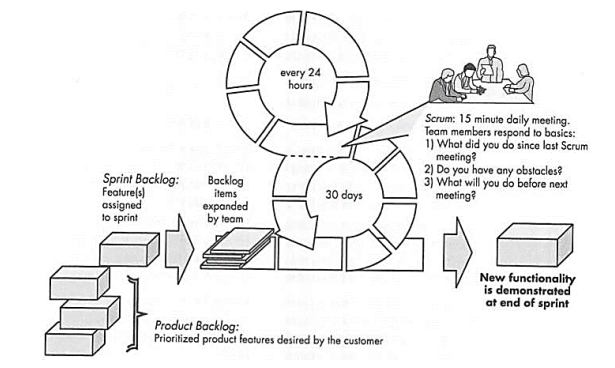
\includegraphics [width = 12.5cm, height= 8cm]{gambar/alur_proses_scrum}}
\caption{Alur Proses Scrum}
\label{alur_proses_scrum}
\end{figure}	

\par Menurut \cite{pressman2010}, di setiap tahap pengembangan, terjadi aktivitas kerja yang terlingkup di dalam suatu pola proses yang dinamakan sprint. Setiap pola proses yang terjadi, akan terdapat seperangkat kegiatan berikut: 

\begin{enumerate}[a.]
\item \textit{Backlog}
 \par Sebuah rincian prioritas pada fitur-fitur yang akan dibangun pada suatu proyek. Isi pada fitur dapat ditambahkan setiap saat. 
 \item \textit{Sprints} 
 \par Kumpulan aktivitas kerja yang dilakukan untuk memenuhi kebutuhan yang ditetapkan dalam backlog dan harus diselesaikan pada waktu yang telah ditentukan. Perubahan tidak dapat dilakukan pada proses sprintsehingga setiap tim akan bekerja di dalam lingkungan yang stabil. 
 \item \textit{Scrum Meeting} 
 \par Pertemuan yang dilakukan setiap hari oleh tim scrum untuk membahas apa yang telah dikerjakan sejak pertemuan terakhir, merencanakan dan membahas masalah-masalah yang ada (biasanya 15 menit).
 \item \textit{Demos} 
 \par Menujukan hasil fungsionalitas yang telah diimplementasikan sehingga dapat dievaluasi oleh pengguna. 
 Demo harus berupa fitur-fitur yang telah diselesaikan sesuai dengan waktu yang telah ditetapkan. 
\end{enumerate}

\section{\uppercase{Black Box Testing}}
Pengujian \textit{blackbox (blackbox testing)} adalah salah satu metode pengujian perangkat lunak yang berfokus pada sisi fungsionalitas, khususnya pada input dan output aplikasi (apakah sudah sesuai dengan apa yang diharapkan atau belum). Tahap pengujian atau testing merupakan salah satu tahap yang harus ada dalam sebuah siklus pengembangan perangkat lunak (selain tahap perancangan atau desain). \citep{iskandaria2012}. Menurut \cite{shihab2011} kategori kesalahan/error yang akan diketahui melalui black box testing :

\begin{itemize}
\item Fungsi yang hilang atau tak benar/salah
\item Error dari antar-muka/interface
\item Error dari struktur data atau akses eksternal database
\item Error dari kinerja atau tingkah laku/perform
\item Error dari inisialisasi dan terminasi
\end{itemize}


\section{\uppercase{SYSTEM USABILITY SCALE (SUS)}}
\textit{System Usability Scale (SUS)} merupakan metode pengujian usability suatu sistem secara sederhana dengan sepuluh skala yang memberikan pandangan secara menyeluruh dari evaluasi tujuan kebergunaan. SUS berupa skala Likert yang sederhana dengan responden diharuskan penjawab tingkat kesetujuan dan ketidaksetujuan daam skala 5 atau 7 poin. SUS dapat dipercaya, skala usability dengan biaya rendah yang dapat digunakan untuk pengujian sistem usability secara global.

\par \textit{System Usability Scale (SUS)} menghasilkan satu nomor mewakili ukuran gabungan dari kegunaan keseluruhan dari Sistem yang dipelajari. Perhatikan bahwa skor untuk setiap item yang tidak bermakna pada mereka sendiri. Untuk menghitung skor SUS, sum pertama kontribusi skor dari setiap item. Setiap item kontribusi skor akan berkisar dari 0 sampai 4. Untuk item 1,3,5,7, dan 9 kontribusi skor adalah skala posisi dikurangi 1. Untuk item 2,4,6,8 dan 10, kontribusi adalah 5 minus posisi skala. Kalikan jumlah nilai sebesar 2,5 untuk mendapatkan nilai keseluruhan SU. Skor SUS memiliki berbagai 0 sampai 100 \citep{brooke2007}.


%-----------------------------------------------------------------------------%

% Baris ini digunakan untuk membantu dalam melakukan sitasi
% Karena diapit dengan comment, maka baris ini akan diabaikan
% oleh compiler LaTeX.

\fancyhf{} 
\fancyfoot[R]{\thepage}

\begin{comment}
\bibliography{daftar-pustaka}
\end{comment}
